\newpage	
	Une variante de \gls{vnm} , 
	\newacronym{dsm}{DSM}{Dense SubGraph Mining}	
	\gls{dsm}, a été proposée par Hernandez et Navarro \citep{hernandez2014compressed}. Comme première contribution, ils augmentent les types de structures découvertes dans la phase de clustering pour englober aussi: les cliques, les bi-cliques. L'extraction de motifs cette fois-ci n'est pas basée sur un parcours des feuilles vers la racine mais l'inverse où  l'ensemble des sommets finaux des liens du motifs est constitué des étiquettes des nœuds de l'arbre inclues dans le chemin de la racine vers la feuille et  les sommets initiaux sont la liste des sommets inclus dans le nœud feuille. 
				%%Noublie pas revient vers la source 
				Leur deuxième contribution consiste en une hybridation dans le but de représenter le graphe en sortie à l'aide de structures compactes. Une première approche proposée est d'utiliser les  k2-trees \citep{brisaboa2009k}  qui donnent la représentation la plus compacte.  
				La deuxième hybridation consiste en une nouvelle structure proposée par les auteurs.\\
				
				
				
				\begin{figure}[!h]
					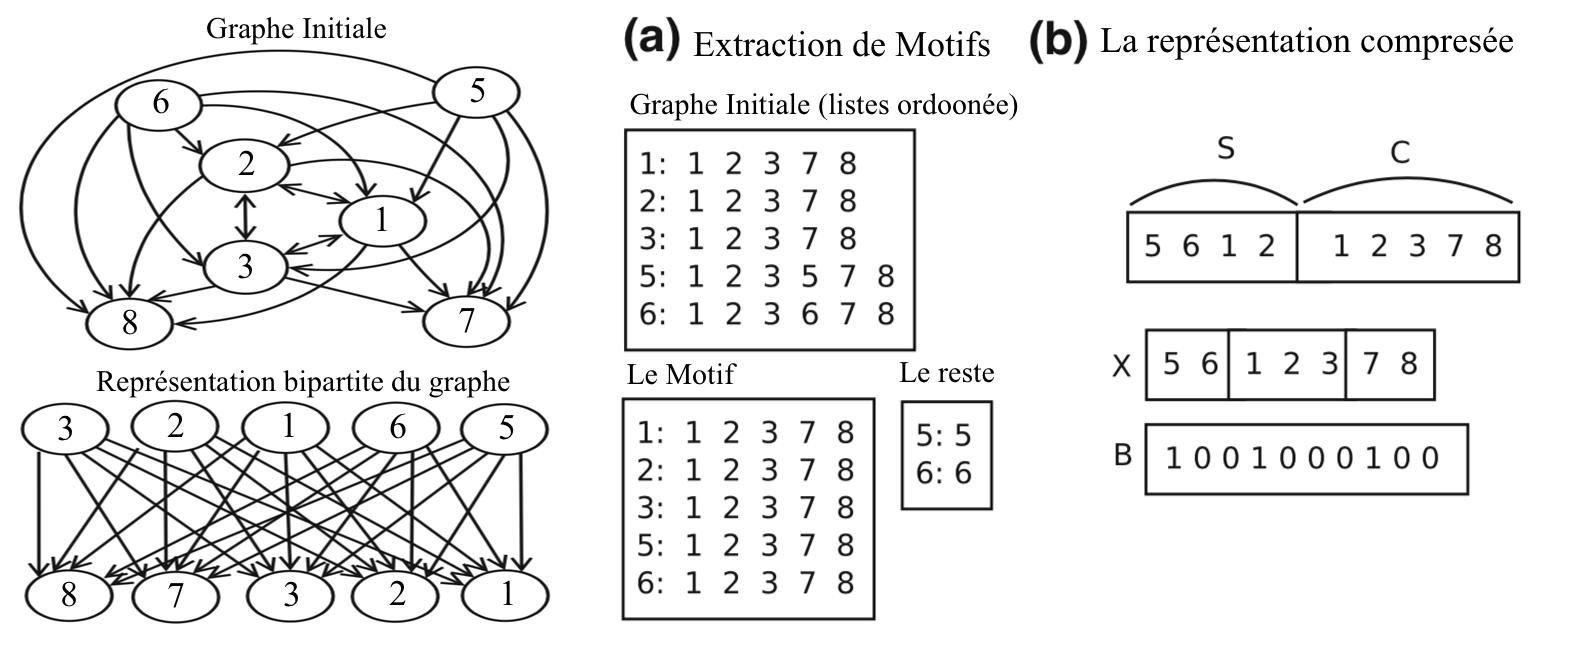
\includegraphics[scale=0.23]{ressources/image/VNM2_exemple.png} 
					\caption{Exemple d'exécution de DSM}
					\label{SDM}
				\end{figure}
			